\chapter{Results}
This chapter presents the experimental results and analyses of the Pix2Pix model across multiple evaluation settings. Both quantitative and qualitative assessments are conducted to examine the model’s performance in translating Sentinel-1 SAR imagery into full-spectrum Sentinel-2 optical outputs. The primary objectives are to evaluate the model’s reconstruction capability, investigate the influence of training data scale, and assess its ability in cloud removal.
Given the high sensitivity of GAN-based frameworks to hyperparameter choices, several experimental configurations were explored to ensure stable convergence and high-quality reconstructions. Initial experiments were performed using 20\% of the winter subset to efficiently test different settings. However, the results obtained with this limited data were unsatisfactory. Following the hypothesis that training on a larger dataset would enhance performance, the model was subsequently trained on the entire winter subset, consisting of 31,825 image pairs.
Beyond the dataset-scale comparison, additional analyses examine the reconstruction quality across individual Sentinel-2 bands and evaluate the model’s ability to remove cloud contamination using the complementary SEN12-MS-CR dataset. Together, these experiments provide a comprehensive view of the model’s spatial, spectral, and perceptual performance under realistic remote-sensing scenarios.

\section{Results on 20\% of the Winter Subset}
In the initial stage of experimentation, only 20\% of the data were used for training. From the 31,825 image pairs in the winter subset, 3,215, 981, and 981 pairs were allocated for training, validation, and testing, respectively. The model was trained to reconstruct the full optical spectrum consisting of 13 bands, using the dual VV and VH polarization SAR data as input.
The preprocessing steps, training pipeline, and hyperparameter settings were identical to those described previously and were applied unchanged to the experiments on the full winter subset. Moreover, the training was conducted using the full combination of loss functions, as discussed in Section~\ref{subsec:losses}.

\begin{figure}[h!]
    \centering
    \setlength{\tabcolsep}{2pt} % horizontal padding between columns (same as ablation)
    \renewcommand{\arraystretch}{1.0} % vertical padding (same as ablation)

    \begin{tabular}{c *{3}{c}}
        % ------------------- Row 1 -------------------
        \textbf{(a)} &
        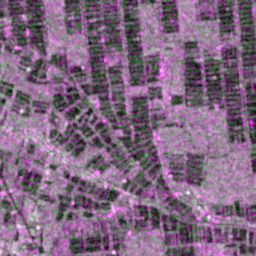
\includegraphics[width=0.2\textwidth, height=0.2\textheight, keepaspectratio]{img/qualitative-20/sample_1/sar.png} &
        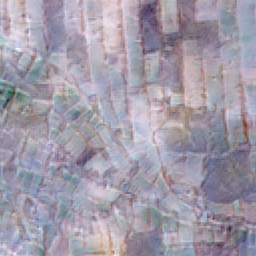
\includegraphics[width=0.2\textwidth, height=0.2\textheight, keepaspectratio]{img/qualitative-20/sample_1/gen.png} &
        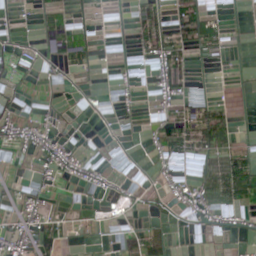
\includegraphics[width=0.2\textwidth, height=0.2\textheight, keepaspectratio]{img/qualitative-20/sample_1/gt.png} \\
        % ------------------- Row 2 -------------------
        \textbf{(b)} &
        \includegraphics[width=0.2\textwidth, height=0.2\textheight, keepaspectratio]{img/qualitative-20/sample_3/sar.png} &
        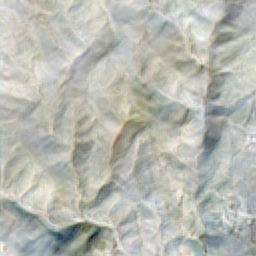
\includegraphics[width=0.2\textwidth, height=0.2\textheight, keepaspectratio]{img/qualitative-20/sample_3/gen.png} &
        \includegraphics[width=0.2\textwidth, height=0.2\textheight, keepaspectratio]{img/qualitative-20/sample_3/gt.png} \\
        \textbf{(c)} &
        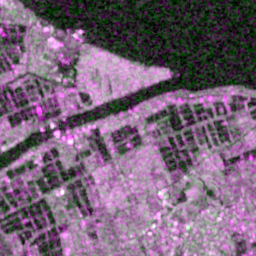
\includegraphics[width=0.2\textwidth, height=0.2\textheight, keepaspectratio]{img/qualitative-20/sample_5/sar.png} &
        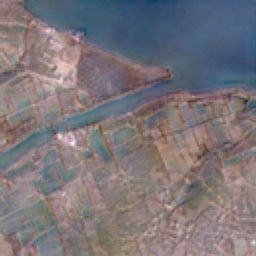
\includegraphics[width=0.2\textwidth, height=0.2\textheight, keepaspectratio]{img/qualitative-20/sample_5/gen.png} &
        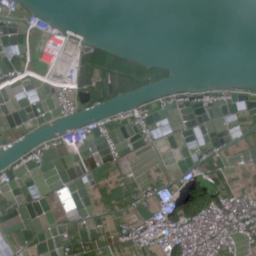
\includegraphics[width=0.2\textwidth, height=0.2\textheight, keepaspectratio]{img/qualitative-20/sample_5/gt.png} \\
        % ------------------- Row 6 -------------------
        \textbf{(d)} &
        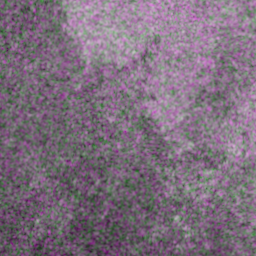
\includegraphics[width=0.2\textwidth, height=0.2\textheight, keepaspectratio]{img/qualitative-20/sample_7/sar.png} &
        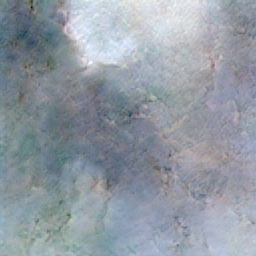
\includegraphics[width=0.2\textwidth, height=0.2\textheight, keepaspectratio]{img/qualitative-20/sample_7/gen.png} &
        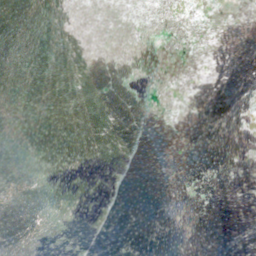
\includegraphics[width=0.2\textwidth, height=0.2\textheight, keepaspectratio]{img/qualitative-20/sample_7/gt.png} \\
    \end{tabular}

    \caption[Qualitative results of 20\% training winter subset]{%
    Qualitative results of 20\% training winter subset.
    Columns: 
    \textbf{(i)}~SAR input (pseudo RGB), 
    \textbf{(ii)}~model-generated optical image, 
    \textbf{(iii)}~ground-truth Sentinel-2 image. All optical images throughout this thesis are depicted in RGB (B4, B4, B2) batch.}
    \label{fig:qualitative_results_20}
\end{figure}

Examining the qualitative results in Figure~\ref{fig:qualitative_results_20}, the model successfully captures large-scale structural patterns such as boundaries, edges, and terrain formations. However, it struggles to reproduce fine-grained details and textural content. For instance, in row~(a), the boundaries of the agricultural fields are well preserved, but the internal texture of the fields is poorly reconstructed. Similarly, in row~(b), the terrain structure is correctly represented, yet the elevation contrast and depth variation are not accurately reproduced. In row~(c), the coastline and water boundaries are distinctly captured, whereas the urban area in the bottom-right corner appears blurred and lacks definition. Lastly, in row~(d), since the corresponding SAR input contains limited structural information, the generated optical output deviates substantially from the ground truth, indicating the model’s reduced ability to infer fine details in textureless regions.


Overall, these observations, together with the quantitative results presented in Table~\ref{tab:quantitative_result_20}, confirm that the model effectively learns the underlying SAR-to-optical mapping and that an optimal training configuration was achieved. While the Pix2Pix model demonstrates strong capability in capturing global spatial correspondences, it exhibits limitations in synthesizing fine textures, particularly within homogeneous or low-contrast regions of the SAR input. Furthermore, the inherent differences in sensing mechanisms and physical characteristics between SAR and optical imagery pose additional challenges for accurately reconstructing fine spatial and spectral details. Motivated by these findings, it was hypothesized that model performance could be enhanced through training on a larger-scale dataset. To validate this hypothesis, the model was subsequently trained on the complete winter subset, and the corresponding results are presented in the following section

\begin{table}[h!]
\centering
\caption[Quantitative results of 20\% training winter subset]{Quantitative results of the training on 20\% of the winter subset.}
\begin{tabular}{lccccc}
\toprule
\textbf{SSIM} & \textbf{PSNR (dB)} & \textbf{LPIPS} & \textbf{SAM (°)} & \textbf{MAE} & \textbf{RMSE} \\
\midrule
0.859 & 27.65 & 0.224 & 6.71 & 195.30 & 381.57 \\
\bottomrule
\end{tabular}
\label{tab:quantitative_result_20}
\end{table}

\section{Results on the Full Winter Subset}
GAN-based models generally require large amounts of training data to achieve high-quality image generation, particularly when using mono-temporal SAR imagery as input for translation to optical domains~\cite{sar_2_opt_CGAN_survey_taxonomy}, and especially when reconstructing the full spectral range. Since training on only 20\% of the dataset did not yield satisfactory results, an additional experiment was conducted using the full winter subset, which comprises 31,825 samples divided in an 8:1:1 ratio for training, validation, and testing. This corresponds to approximately 25,460 samples for training and 3,180 samples each for validation and testing. The data preprocessing procedure, training pipeline, and hyperparameters were kept identical to those used in the 20\% experiment to ensure that the effect of training data size was isolated and directly evaluated.

The model required approximately 25$\sim$hours to complete 150~epochs of training. The experimental hypothesis was confirmed: increasing the size of the training dataset led to a clear improvement in model performance. As shown in Table~\ref{tab:quantitative_result_scale}, expanding the training data from 20\% to the full winter subset resulted in substantial gains across all evaluation metrics. In particular, the LPIPS score decreased from 0.224 to 0.173, indicating that the model trained on the full dataset produced outputs with higher perceptual similarity to the ground truth. Likewise, the median SAM value dropped from 6.71° to 4.41°, demonstrating a notable enhancement in spectral consistency across all bands. Furthermore, PSNR increased by approximately 5$\sim$dB, while MAE and RMSE decreased by more than 25\%, confirming the strong positive effect of data scale on reconstruction quality.

\begin{table}[h!]
    \centering
    \caption[Quantitative results for different training data scales: 20\% \& 100\%]{Quantitative results of training on 20\% and 100\% of the winter subset. Arrows ($\uparrow$ / $\downarrow$) indicate whether higher or lower values denote better performance, respectively.}
    \begin{tabular}{lcccccc}
        \toprule
        \textbf{Training Data} & \textbf{SSIM $\uparrow$} & \textbf{PSNR (dB) $\uparrow$} & \textbf{LPIPS $\downarrow$} & \textbf{SAM (°) $\downarrow$} & \textbf{MAE $\downarrow$} & \textbf{RMSE $\downarrow$} \\
        \midrule
        20\% of subset         & 0.859                    & 27.65                         & 0.224                       & 6.71                          & 195.30                    & 381.57                     \\
        100\% of subset        & \textbf{0.888}           & \textbf{32.63}                & \textbf{0.173}              & \textbf{4.41}                 & \textbf{140.72}           & \textbf{233.69}            \\
        \bottomrule
    \end{tabular}
    \label{tab:quantitative_result_scale}
\end{table} 
Similarly, the image reconstruction quality improves noticeably with a larger training dataset. Qualitative examples are shown in Figure~\ref{fig:qualitative_results_100_20}. The model trained on the full winter subset not only better preserves the structural details of the reference images but also achieves markedly enhanced color fidelity, as evident in column (a). In the urban scene (b), it accurately reconstructs the city layout and successfully delineates the river traversing the area. Furthermore, compared to the model trained on only 20\% of the data, the full-data model better captures surface relief and elevation depth, as illustrated in (c).

These qualitative and quantitative improvements demonstrate the capability of the Pix2Pix model to reconstruct optical imagery solely from SAR data. Furthermore, expanding the volume and diversity of the training dataset enables the model to more effectively learn the perceptual and spectral characteristics of the optical domain, thereby producing reconstructions that are both more realistic and color-consistent.

\begin{figure}[h!]
    \centering
    \setlength{\tabcolsep}{2pt} % horizontal padding between columns (same as ablation)
    \renewcommand{\arraystretch}{1.0} % vertical padding (same as ablation)

    \begin{tabular}{c *{4}{c}}
        % ------------------- Row 1 -------------------
        \textbf{(a)} &
        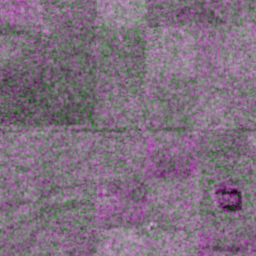
\includegraphics[width=0.2\textwidth, height=0.2\textheight, keepaspectratio]{img/qualitative-20-full/sample_1/sar.png} &
        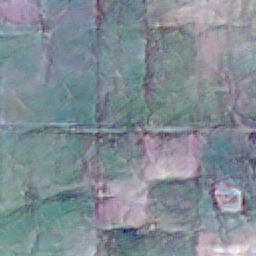
\includegraphics[width=0.2\textwidth, height=0.2\textheight, keepaspectratio]{img/qualitative-20-full/sample_1/gen_0.2.png} &
        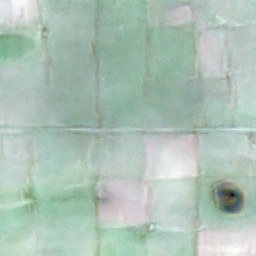
\includegraphics[width=0.2\textwidth, height=0.2\textheight, keepaspectratio]{img/qualitative-20-full/sample_1/gen_full.png} &
        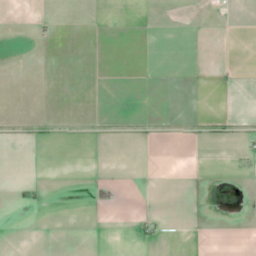
\includegraphics[width=0.2\textwidth, height=0.2\textheight, keepaspectratio]{img/qualitative-20-full/sample_1/gt.png} \\
        % ------------------- Row 2 -------------------
        \textbf{(b)} &
        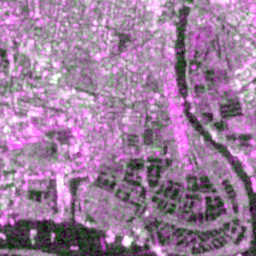
\includegraphics[width=0.2\textwidth, height=0.2\textheight, keepaspectratio]{img/qualitative-20-full/sample_2/sar.png} &
        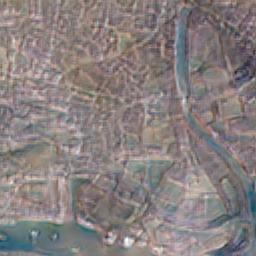
\includegraphics[width=0.2\textwidth, height=0.2\textheight, keepaspectratio]{img/qualitative-20-full/sample_2/gen_0.2.png} &
        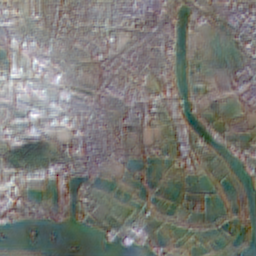
\includegraphics[width=0.2\textwidth, height=0.2\textheight, keepaspectratio]{img/qualitative-20-full/sample_2/gen_full.png} &
        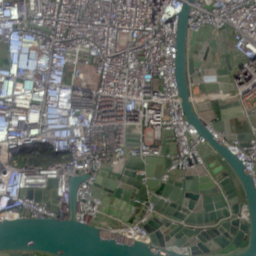
\includegraphics[width=0.2\textwidth, height=0.2\textheight, keepaspectratio]{img/qualitative-20-full/sample_2/gt.png} \\
        \textbf{(c)} &
        \includegraphics[width=0.2\textwidth, height=0.2\textheight, keepaspectratio]{img/qualitative-20-full/sample_3/sar.png} &
        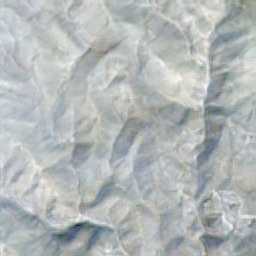
\includegraphics[width=0.2\textwidth, height=0.2\textheight, keepaspectratio]{img/qualitative-20-full/sample_3/gen_0.2.png} &
        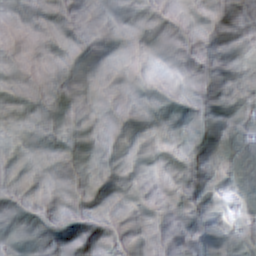
\includegraphics[width=0.2\textwidth, height=0.2\textheight, keepaspectratio]{img/qualitative-20-full/sample_3/gen_full.png} &
        \includegraphics[width=0.2\textwidth, height=0.2\textheight, keepaspectratio]{img/qualitative-20-full/sample_3/gt.png} \\
        % ------------------- Row 6 -------------------
        \textbf{(d)} &
        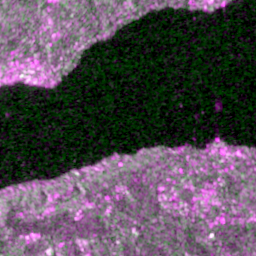
\includegraphics[width=0.2\textwidth, height=0.2\textheight, keepaspectratio]{img/qualitative-20-full/sample_4/sar.png} &
        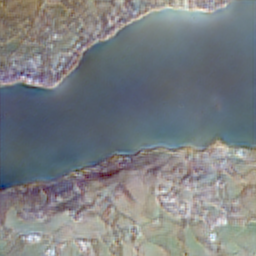
\includegraphics[width=0.2\textwidth, height=0.2\textheight, keepaspectratio]{img/qualitative-20-full/sample_4/gen_0.2.png} &
        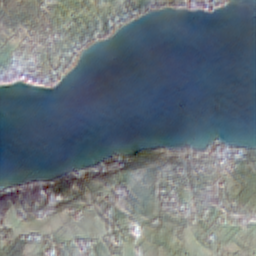
\includegraphics[width=0.2\textwidth, height=0.2\textheight, keepaspectratio]{img/qualitative-20-full/sample_4/gen_full.png} &
        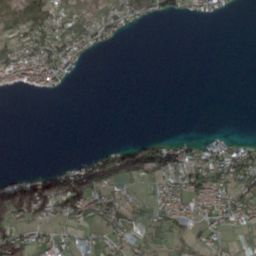
\includegraphics[width=0.2\textwidth, height=0.2\textheight, keepaspectratio]{img/qualitative-20-full/sample_4/gt.png} \\
    \end{tabular}

    \caption[Qualitative results for different training data scales: 20\% \& 100\%]{%
    Qualitative comparison of models trained on 20\% and 100\% of the dataset. 
    Columns: \textbf{(i)}~SAR input (pseudo-RGB), 
    \textbf{(ii)}~generated optical image from 20\% training, 
    \textbf{(iii)}~generated optical image from 100\% training, and 
    \textbf{(iv)}~ground-truth Sentinel-2 image. All optical images are depicted in RGB (B4, B4, B2) batch.}
    \label{fig:qualitative_results_100_20}
\end{figure}

\section{Results Across Individual Optical Bands}
Another objective of this work was to assess the model’s ability to reliably reconstruct each optical band individually and to evaluate the extent of its accuracy across the spectrum. 
For this purpose, the model trained on the full winter subset was evaluated separately for all Sentinel-2 bands, and the corresponding results are summarized in Table~\ref{tab:per_band_validation}.
When comparing the reconstruction quality across individual bands, the focus is placed on the unitless SSIM metric. Other metrics such as MAE or RMSE are not directly comparable between bands, as they depend on the absolute magnitude and statistical distribution of reflectance values, which differ across spectral ranges. In contrast, SSIM measures local structural similarity based on relative intensity patterns rather than absolute values. While not entirely invariant to scale differences, SSIM provides a more robust and interpretable basis for cross-band comparison in this context.

\begin{table}[h!]
\centering
\caption[Per-band validation results for full dataset training]{%
Per-band quantitative validation results of the Pix2Pix model trained on the full winter subset. Each Sentinel-2 band’s central wavelength, spectral designation, and native spatial resolution are listed for reference. Best results are highlighted in \textcolor{green!50!black}{green} and worst in \textcolor{red!70!black}{red}.}
\resizebox{0.9\textwidth}{!}{%
\begin{tabular}{lcccc}
\toprule
\textbf{Band} & \textbf{PSNR (dB) $\uparrow$} & \textbf{SSIM $\uparrow$} & \textbf{Central Wavelength [nm]} & \textbf{Spectral / Resolution [m]} \\
\midrule
B1   &  36.53  &  \cellcolor{green!15}\textbf{0.9758} & 443  & Aerosols / 60 \\
B2   &  \cellcolor{green!15}\textbf{37.49}  &  0.9506 & 490  & Blue / 10 \\
B3   &  35.67  &  0.9199 & 560  & Green / 10 \\
B4   &  32.84  &  0.8639 & 665  & Red / 10 \\
B5   &  33.68  &  0.9007 & 705  & Red Edge / 20 \\
B6   &  31.62  &  0.8536 & 740  & Red Edge / 20 \\
B7   &  30.37  &  0.8253 & 783  & Red Edge / 20 \\
B8   &  \cellcolor{red!15}\textit{29.62}  &  \cellcolor{red!15}\textit{0.7738} & 842  & NIR / 10 \\
B8A  &  29.62  &  0.8071 & 865  & Red Edge / 20 \\
B9   &  33.99  &  0.9388 & 945  & Water Vapour / 60 \\
B10  &  32.12  &  0.9386 & 1375 & Cirrus / 60 \\
B11  &  29.92  &  0.8309 & 1610 & SWIR / 20 \\
B12  &  31.48  &  0.8586 & 2190 & SWIR / 20 \\
\bottomrule
\end{tabular}% 
}
\label{tab:per_band_validation}
\end{table}
Notably, Band~8 (NIR), despite its native spatial resolution of 10~m, exhibits the lowest reconstruction performance among all spectral bands, including those with coarser resolutions, as illustrated in Figure~\ref{fig:ssim_per_band}. This indicates a weaker correlation between SAR backscatter and NIR reflectance compared to other spectral regions, likely due to their differing sensitivities to surface structure and vegetation properties. This limitation may also stem from the use of winter-only training samples, where vegetation-related information captured by the NIR band is comparatively scarce. In contrast, the 60~m atmospheric correction bands—B1 (Aerosols), B9 (Water Vapour), and B10 (Cirrus)—are reconstructed more reliably, with B1 achieving the highest SSIM overall. Their smoother spectral characteristics and lower spatial variability likely facilitate more stable and accurate predictions, even after resampling to 10~m.
\begin{figure}[h!]
\centering
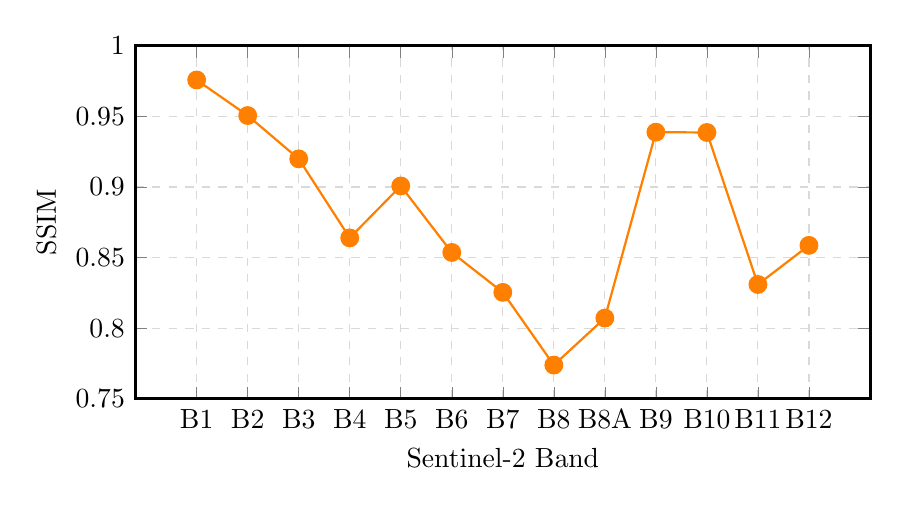
\begin{tikzpicture}
\begin{axis}[
    width=0.9\textwidth,
    height=0.5\textwidth,
    xlabel={Sentinel-2 Band},
    ylabel={SSIM},
    ymin=0.75, ymax=1.0,
    ytick distance=0.05,
    xtick=data,
    xticklabels={B1,B2,B3,B4,B5,B6,B7,B8,B8A,B9,B10,B11,B12},
    grid=major,
    grid style={dashed,gray!30},
    every axis plot/.append style={thick, mark=*},
    mark size=3pt,
    line width=1pt,
]

\addplot[
    color=orange,
    mark=*,
    mark options={fill=orange},
]
coordinates {
    (1,0.9758)
    (2,0.9506)
    (3,0.9199)
    (4,0.8639)
    (5,0.9007)
    (6,0.8536)
    (7,0.8253)
    (8,0.7738)
    (9,0.8071)
    (10,0.9388)
    (11,0.9386)
    (12,0.8309)
    (13,0.8586)
};

\end{axis}
\end{tikzpicture}
\caption[Per-band SSIM for the Pix2Pix model]{Per-band SSIM for the Pix2Pix model trained on the full winter subset.}
\label{fig:ssim_per_band}
\end{figure}

It is worth noting, however, that these findings contradict those reported in~\cite{CR_SEN2_dRNN}, where the authors observed the 10~m and 20~m bands to achieve the highest reconstruction quality, while the 60~m bands performed the worst. Their experiments were conducted on the full SEN12-MS-CR dataset, which may account for the differing behavior observed in the present study.

To visually complement the quantitative assessment, representative grayscale examples for each Sentinel-2 band are provided in Appendix~\ref{appendix:bandwise_results}. Each example illustrates the generated band alongside its corresponding ground-truth reference, enabling a direct visual evaluation of the reconstruction quality and spatial consistency across the spectrum.

\newpage

\section{Results on Cloud Removal}
\label{sec:cloud_removal}
Cloud contamination remains one of the most persistent challenges in the field of remote sensing. To evaluate the model’s capability to address this issue, the model trained on the complete winter subset of the SEN12-MS dataset was assessed using the complementary SEN12-MS-CR dataset (see Section~\ref{sec:datasets}). The SEN12-MS-CR dataset consists of triplets comprising SAR images, cloud-contaminated optical images, and their corresponding cloud-free optical references, covering identical geographic regions across all 13 Sentinel-2 spectral bands.
For quantitative evaluation, a subset of 2,000 samples from the winter portion of the SEN12-MS-CR dataset was used. The evaluation data underwent identical preprocessing and clipping procedures as described in Section~\ref{subsec:preprocessing}, ensuring consistency with the model’s training conditions.

\begin{table}[h!]
    \centering
    \caption[Quantitative results on cloud removal]{Quantitative evaluation of different models trained on the full winter subset of the SEN12-MS dataset, assessed on the complementary SEN12-MS-CR dataset for the \textbf{cloud removal} task.}
    \begin{tabular}{lcccc}
        \toprule
        \textbf{Model}               & \textbf{SSIM $\uparrow$} & \textbf{PSNR (dB) $\uparrow$} & \textbf{LPIPS $\downarrow$} & \textbf{SAM (°) $\downarrow$} \\
        \midrule
        DSen2-CR~\cite{CR_SEN2_dRNN} & 0.878                    & --                            & --                          & 8.07                          \\
        FAT~\cite{c_guided_fus_s2ot} & 0.880                    & 31.85                         & --                          & 4.19                          \\
        DiffCR~\cite{DiffCR} (SOTA)  & \textbf{0.902}           & 31.77                         & --                          & 5.82                          \\
        Pix2Pix (This Thesis)        & 0.899                    & \textbf{33.65}                & \textbf{0.152}              & \textbf{3.86}                 \\
        \bottomrule
    \end{tabular}
    \label{tab:quantitative_result_cr}
\end{table}

The quantitative results presented in Table~\ref{tab:quantitative_result_cr} demonstrate that the model attains robust and high-quality performance in cloud removal on the SEN12-MS-CR dataset, despite not being explicitly trained for this task or on this dataset. Notably, the reconstruction accuracy surpasses that achieved on the model’s own training subset (SEN12-MS) across all evaluated metrics. The spectral fidelity, measured by the SAM, improved by approximately one degree, indicating better preservation of spectral characteristics. Remarkably, the trained Pix2Pix model even outperforms several specialized approaches, including DiffCR~\cite{DiffCR}, the current state-of-the-art model for cloud removal on SEN12-MS-CR—an outcome that was beyond the original scope of this thesis. This result is particularly significant given that Pix2Pix is typically employed as a baseline model in related studies and is often reported to yield the lowest performance among compared methods 

The qualitative results shown in Figure~\ref{fig:qualitative_results_cloud_removal} further illustrate the model’s effectiveness in removing cloud contamination. The model successfully reconstructs cloud-free optical imagery from the corresponding SAR inputs, even when the reference optical images are heavily obscured. As seen in rows (a) and (b), the model accurately restores regions affected by thin cloud cover while preserving structural and textural details. In partially occluded cases, illustrated in (c) and (d), the reconstructed outputs maintain clear boundaries, sharp edges, and consistent color representation. Remarkably, even for fully cloud-covered scenes, as in (e), the model generates realistic optical imagery and reliably reproduces urban and structural features.

\begin{figure}[h!]
    \centering
    \setlength{\tabcolsep}{2pt} % horizontal padding between columns (same as ablation)
    \renewcommand{\arraystretch}{1.0} % vertical padding (same as ablation)

    \begin{tabular}{c *{4}{c}}
        % ------------------- Row 1 -------------------
        \textbf{(a)} &
        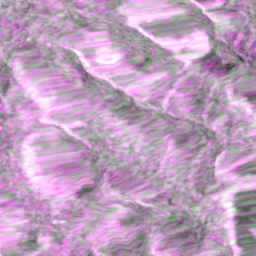
\includegraphics[width=0.2\textwidth, height=0.2\textheight, keepaspectratio]{img/cloud_removal/sample_000881_sar_pseudo.png} &
        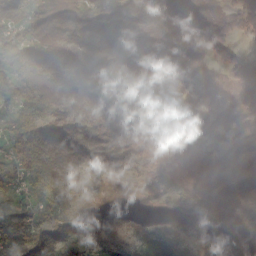
\includegraphics[width=0.2\textwidth, height=0.2\textheight, keepaspectratio]{img/cloud_removal/sample_000881_cloudy_rgb.png} &
        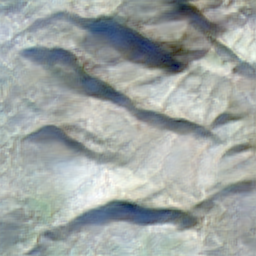
\includegraphics[width=0.2\textwidth, height=0.2\textheight, keepaspectratio]{img/cloud_removal/sample_000881_pred_rgb.png} &
        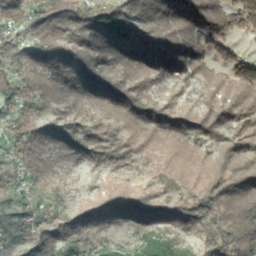
\includegraphics[width=0.2\textwidth, height=0.2\textheight, keepaspectratio]{img/cloud_removal/sample_000881_true_rgb.png} \\
        % ------------------- Row 2 -------------------
        \textbf{(b)} &
        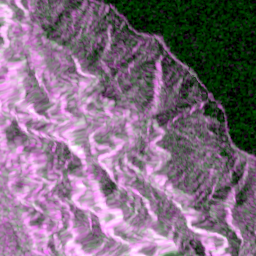
\includegraphics[width=0.2\textwidth, height=0.2\textheight, keepaspectratio]{img/cloud_removal/sample_000683_sar_pseudo.png} &
        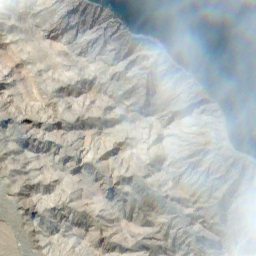
\includegraphics[width=0.2\textwidth, height=0.2\textheight, keepaspectratio]{img/cloud_removal/sample_000683_cloudy_rgb.png} &
        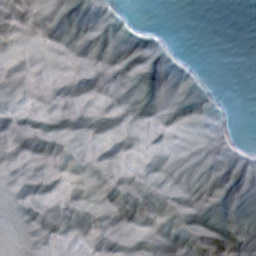
\includegraphics[width=0.2\textwidth, height=0.2\textheight, keepaspectratio]{img/cloud_removal/sample_000683_pred_rgb.png} &
        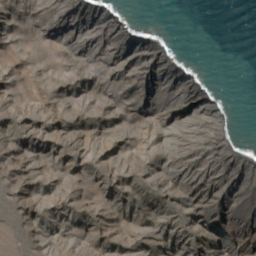
\includegraphics[width=0.2\textwidth, height=0.2\textheight, keepaspectratio]{img/cloud_removal/sample_000683_true_rgb.png} \\
        \textbf{(c)} &
        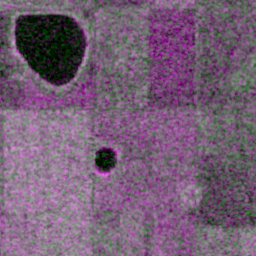
\includegraphics[width=0.2\textwidth, height=0.2\textheight, keepaspectratio]{img/cloud_removal/sample_001114_sar_pseudo.png} &
        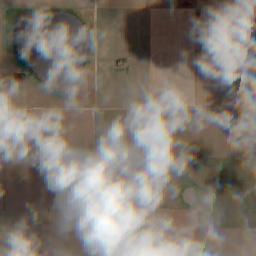
\includegraphics[width=0.2\textwidth, height=0.2\textheight, keepaspectratio]{img/cloud_removal/sample_001114_cloudy_rgb.png} &
        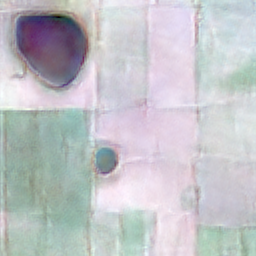
\includegraphics[width=0.2\textwidth, height=0.2\textheight, keepaspectratio]{img/cloud_removal/sample_001114_pred_rgb.png} &
        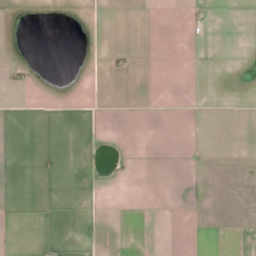
\includegraphics[width=0.2\textwidth, height=0.2\textheight, keepaspectratio]{img/cloud_removal/sample_001114_true_rgb.png} \\
        \textbf{(d)} &
        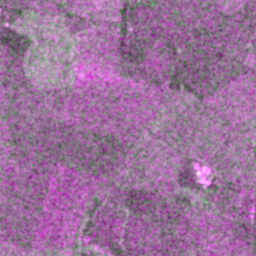
\includegraphics[width=0.2\textwidth, height=0.2\textheight, keepaspectratio]{img/cloud_removal/sample_000013_sar_pseudo.png} &
        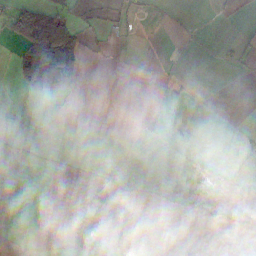
\includegraphics[width=0.2\textwidth, height=0.2\textheight, keepaspectratio]{img/cloud_removal/sample_000013_cloudy_rgb.png} &
        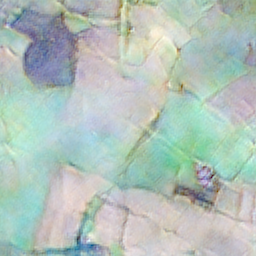
\includegraphics[width=0.2\textwidth, height=0.2\textheight, keepaspectratio]{img/cloud_removal/sample_000013_pred_rgb.png} &
        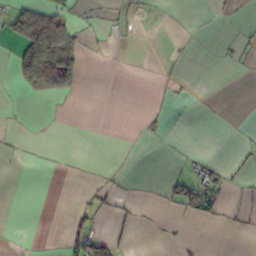
\includegraphics[width=0.2\textwidth, height=0.2\textheight, keepaspectratio]{img/cloud_removal/sample_000013_true_rgb.png} \\
        % ------------------- Row 6 -------------------
        \textbf{(e)} &
        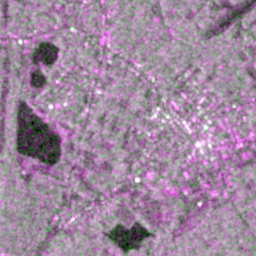
\includegraphics[width=0.2\textwidth, height=0.2\textheight, keepaspectratio]{img/cloud_removal/sample_000150_sar_pseudo.png} &
        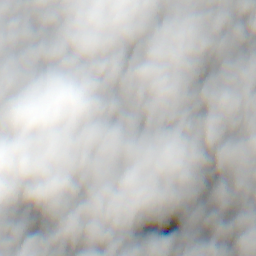
\includegraphics[width=0.2\textwidth, height=0.2\textheight, keepaspectratio]{img/cloud_removal/sample_000150_cloudy_rgb.png} &
        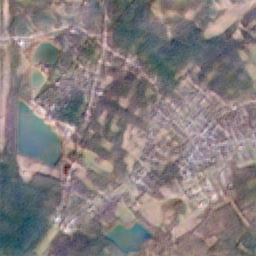
\includegraphics[width=0.2\textwidth, height=0.2\textheight, keepaspectratio]{img/cloud_removal/sample_000150_pred_rgb.png} &
        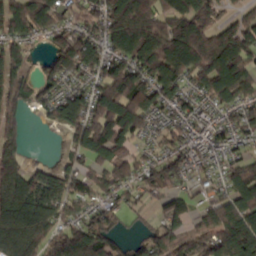
\includegraphics[width=0.2\textwidth, height=0.2\textheight, keepaspectratio]{img/cloud_removal/sample_000150_true_rgb.png} \\
    \end{tabular}

    \caption[Qualitative results on cloud removal]{%
    Qualitative results of the model trained on the full winter subset of the SEN12-MS dataset, evaluated on the complementary SEN12-MS-CR dataset for the \textbf{cloud removal} task.  
    Columns: 
    \textbf{(i)}~SAR input (pseudo-RGB), 
    \textbf{(ii)}~reference cloud-contaminated optical image, 
    \textbf{(iii)}~generated cloud-free optical image, and 
    \textbf{(iv)}~reference cloud-free optical image (ground truth).}
    \label{fig:qualitative_results_cloud_removal}
\end{figure}

Overall, both the qualitative and quantitative results confirm the model’s ability to generate high-quality, cloud-free optical images across all 13 spectral bands solely from SAR inputs, thereby effectively addressing the cloud cover problem. However, since the model was trained exclusively on translating SAR to cloud-free optical images, the thickness or density of the clouds does not appear to influence the reconstruction process. For future work, incorporating both SAR and cloud-contaminated optical inputs to generate cloud-free outputs that more closely mimic the reference images is recommended.
